\section{The MEDEAS model}

\subsection{Overview}

This sections aims at describing the main components of the MEDEAS IAM and its components, with a focus on the parts that are the most relevant in this context.

The project, named "Modelling the Energy Development under Environmental And Socioeconomic constraints", aims at creating a modern computational model to predict the future of the energy systems in Europe, while integrating a wide range of physical and social constraints.

First, the IAMs are depicted, then a high-level description of the MEDEAS model is provided. The third subsection will explain more in depth in a key component of MEDEAS, the energy return on investment. In the fourth subsection, the modelling of the RES in MEDEAS is covered. Finally, the principal scenarios in MEDEAS are presented in the fifth subsection.
% The downside in MEDEAS energy module that will be addressed is its low temporal precision and poor assessment of the flexibility of the energy network. These estimations are based on study \cite{delarue}, that provide general approximations, not accurate prediction deduced from the simulation of the energy network, as done in Dispa-SET. The solution that this work will provide is the integration of the surrogate model for that purpose, that will be in charge of computing better approximation of (mainly) curtailment and lost load.

% For contextualisation, the following description of MEDEAS is written.

\subsection{The MEDEAS integrated assessment models}

MEDEAS is an open-source integrated assessment model (IAM), built to "guide the transition to a low carbon European socio-economy" \cite{medeas-website}.

Integrated assessment models are used to make general purpose analysis, combining aspects from different disciplines, such as economy, environment and energy, land use etc. These kinds of models, once properly defined from a mathematical point of view, can then be simulated by computer, for their result to be analysed.

There is a large variety of IAMs, because there are a lot of ways to model the complex interactions, and the large amount of uncertainties between the different components of a model. Hence, there exist a lot of different approaches to the creation of an IAM.

As a side note, the model being open-source is probably one strength as an IAM, meaning that any expert in one domain may be able to contribute to the project.

As previously quoted from their website, the MEDEAS model has been built with the purpose of guiding decarbonation in Europe. It has been designed to compensate for the flaws of other available IAMs, in order to inform policy makers towards a transition to more carbon-independent, sustainable energy.

MEDEAS is built using the Vensim software, and may be used from the Python programming language through the \href{https://pypi.org/project/pysd/}{\texttt{pySD}} package.

\subsection{Model overview}

MEDEAS funds come from the EU for its Horizon 2020 program, under the "Modelling and analysing the snergy system, its transformation and impacts (social, environmental and economic aspects of the energy system)".

And to do so it models the long-term implications of the decisions made by the society. As one cannot predict them, several hypothesis are needed to fix the choices that will be made. Such a set of hypothesis on the evolution of the long-term policy of the society as a whole is called a scenario.

MEDEAS typically sets the simulation horizon between 1995 and 2060, while for longer term analysis it may be raised up to 2100. It also features different settings:
\begin{itemize}
    \item MEDEAS-W, the global one,
    \item MEDEAS-EU, targeting the European Union,
    \item MEDEAS-AU and MEDEAS-BG, targetting Austria and Bulgaria respectively.
\end{itemize}

The MEDEAS IAM is organized into seven modules, that are economy, energy, energy infrastructures, materials, land use, climate change and socio-environmental impacts indicators. The general structure is illustrated on Figure \ref{fig:medeas-modules}.

\begin{figure}[h]
    \centering
    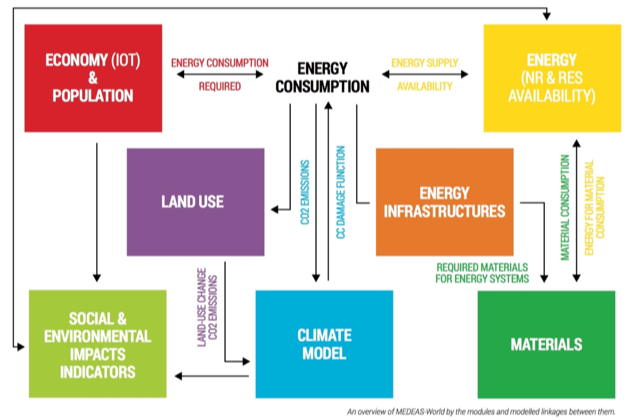
\includegraphics[width=0.9\textwidth]{resources/images/medeas.png}
    \caption{The MEDEAS IAM modules}
    \label{fig:medeas-modules}
\end{figure}

Quite evidently, in this work, the MEDEAS-EU version will be considered, as this is the chosen setting for Dispa-SET, and with an obvious focus on the energy module. 

\subsubsection{System dynamics}

It is formulated using the system dynamics toolset---what Vensim is built for---which is to help the aggregation of the knowledge from different experts from different domains and backgrounds. This will also enable easy modelling of feedback between the different components.

System dynamics is a modeling language, made to obtain understandings of complex and dynamic systems. It acheives using nodes and arrows, corresponding to values and relations between those respectively. The former can be either a stock, a flow or a constant, while the latter makes the link through equations. It is therefore possible to create feedback loops and complex interconnected networks.

System dynamics have been popularized by the \textit{world3} model, used to predict the consequences of long-term policies applied by the society on the planet in the Limits to Growth report \cite{limits-to-growth}.

Needless to say, this approach is far from the linear programming paradigm, that has a too different approach for both to be combined.

\subsection{Energy return on investment}

When having energy consideration in the long term, the energy return on investment (EROI) becomes a key indicator.

It is defined as the ratio of the exploitable energy obtained from some energy resource to the amount of exploitable energy used to get that energy resource \cite{wiki-eroi}.

The EROI is of great importance for the assessment of the energy sources efficiency, providing a measure of how efficient this energy source is to make use of. On most cases, the EROI of RES is lower, meaning a lower energy gain, than fossil fuels'.

It is not to be confused with the net energy gain, that is the difference between the exploitable energy obtained and the exploitable energy invested. The net energy is the amount of energy that has been made exploitable, thus now availible for public consumption. Obviously, its value should be larger than zero for the system to be profitable.

Equations \ref{equation:eroi} and \ref{equation:net-energy} summarize their definitions and the relationship between the two.

\begin{equation}
    EROI=\frac{Energy_{returned}}{Energy_{invested}}
    \label{equation:eroi}
\end{equation}

\begin{equation}
    NetEnergy = Energy_{returned} - Energy_{invested} = Energy_{returned} \Big( 1 - \frac{1}{EROI}\Big)
    \label{equation:net-energy}
\end{equation}

However, this also requires to set a definition on what exactly is the energy invested on the aquisition of an other resource. The MEDEAS model thus provides several EROI values relating to different approaches in this matter \cite{medeas-cost-of-transition}.
\begin{itemize}
    \item Standard EROI, that "includes the direct (i.e. on site) and indirect (i.e. offsite energy needed to make the products used on site) energy requirements to get the energy (e.g. build, operate and maintain a power plant)" \cite{medeas-cost-of-transition}.
    \item Point of use EROI, that includes the energy cost of obtaining and transporting the fuel to the actual location where it will be used by society.
    \item Extended EROI, that " considers the energy required to get, deliver and use a unit of energy, i.e. the energy required to produce the machinery and devices used to build, operate and maintain a power plant or a transportation facility (tank truck, pipeline, etc.) as well as the energy required for exploration, investment, communication, labour, etc. in the energy system" \cite{medeas-cost-of-transition}.
\end{itemize}

In this context, we will focus on the standard EROI.

In MEDEAS, the EROI is dynamically computed, meaning it is an endogenous variable, as the ratio of the exploitable energy delivered to consumers, over the sum of the total energy costs required for operating the plant and the energy costs of handling the variability of the power output and the costs of operating the energy transportation network. The total costs for an operating plant include the building, maintenance and disposal costs.

On Figure \ref{fig:eroi-energy-flows}, a depiction of a high-level energy flow is given. The exploitable energy delivered to consumers is the flow labelled (1), and the operating costs of the plants (2), whereas the costs accounting for the handling of variabilities is labelled (3) and for energy transportation (4). Equation \ref{equation:eroist-medeas}, \ref{equation:eroipou-medeas} and \ref{equation:eroiext-medeas} below shows the MEDEAS' computation of the EROI based on these.

\begin{figure}[h]
    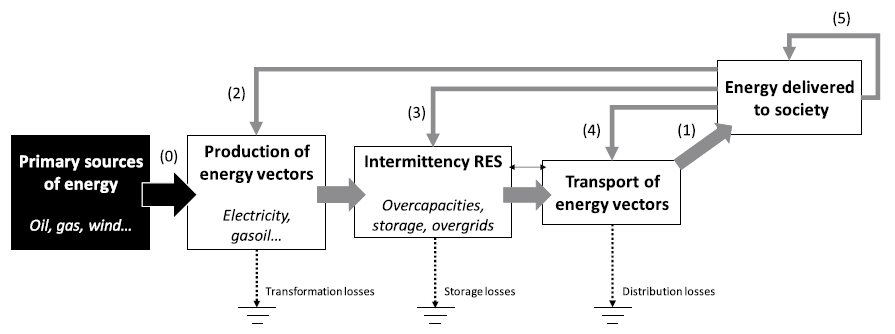
\includegraphics[width=0.9\textwidth]{resources/images/EROI.png}
    \caption{Representation of society's principal energy flows\cite{medeas-eroi}}
    \label{fig:eroi-energy-flows}
\end{figure}

\begin{equation}
    EROI_{st} = \frac{(1)}{(3) + (4)}
    \label{equation:eroist-medeas}
\end{equation}

 \begin{equation}
    EROI_{pou} = \frac{(1)}{(2) + (3) + (4)}
    \label{equation:eroipou-medeas}
 \end{equation}

 \begin{equation}
    EROI_{ext} = \frac{(1)}{(2) + (3) + (4) + (5)}
    \label{equation:eroiext-medeas}
 \end{equation}

Furthermore, MEDEAS \cite{medeas-eroi}:
\begin{itemize}
    \item Assumes the EROI of non renewable energy sources to be constant over time,
    \item Dynamically estimates the EROI of RES producing electricity,
    \item Allocates technologies based on their EROI as a performance measure, meaning that higher EROI RES will be preferred,
    \item Computes overcapacities as a result of an increasing share of VRES endogenously,
    \item Takes additional losses into account for the use of storage units.
\end{itemize}

\subsection{Modelling of RES}

The impacts of the variability of electricity production technologies are tackled in the MEDEAS framework. Indeed, not as extensively as they are in Dispa-SET simulation, what is the whole point of the present work.

\subsubsection{Limitation}

First, it is recalled that the time step used by MEDEAS is quite significant. Is recommended value is 0.03125, expressed as a fraction of a month. This amounts to approximately a day: $0.03125 \times \frac{365.25}{12} = 0.951$.

This value is obviously too high to model extensively daily variations of the power output of solar photovoltaic units, for example.

In the following, the mechanisms implemented by MEDEAS in order to incorporate the RES variability are described.

\subsubsection{Grid extension}

MEDEAS estimates, per MW of VRES, the additional electricity grid extensions required in order to incorporate those in the existing network. The materials needed for these expansions are also computed, what ultimately affects the EROI.

\subsubsection{Storage units}

In MEDEAS, the first storage technology in use is the pumped hydro-storage (PHS). One will notice that it contrasts with the Dispa-SET setting where batteries are used as the main storage technology to act on, mostly by creating new plants. As already discussed before, that is to account for the fact that the european region is almost saturated in terms of PHS, as one could not find suitable location for new units to be built.

An estimation of the storage needs as a function of the VRES share is depicted on Figure \ref{fig:storage-vres} \cite{NREL}.

\begin{figure}[h]
    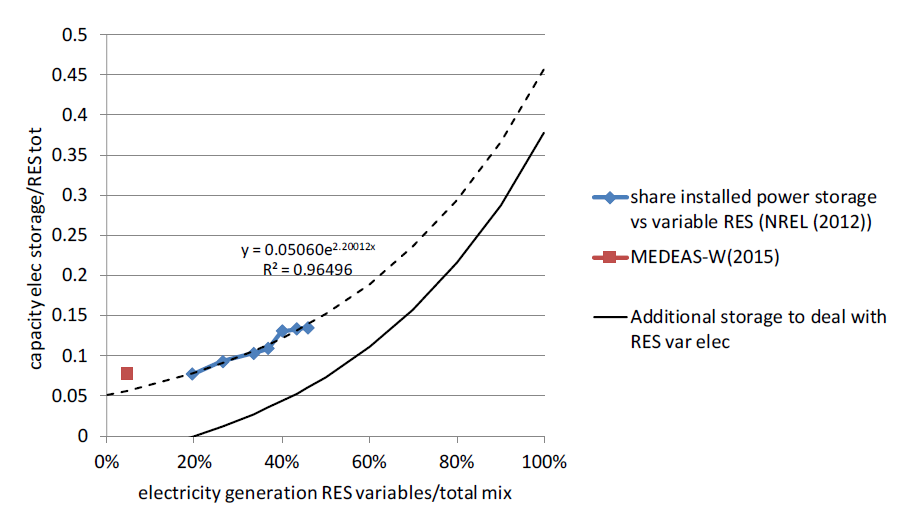
\includegraphics[width=0.8\textwidth]{resources/images/storage.png}
    \caption{Energy storage capacity required as a function of the VRES share according to \cite{NREL}.}
    \label{fig:storage-vres}
\end{figure}

\subsubsection{Dispatchable RES pants}

Here will be describe the evolution of the capacity factor (CF) as the RES share among the electricitym mix changes. The capacity factor is the ratio of the electricity produced by a unit over a period of time $\Delta t$ over the maximum amount of energy that could have been produced. This is represented on Equation \ref{equation:CF-definition}.


\begin{equation}
    CF = \frac{Energy_{produced}}{\Delta t \times PowerCapacity}
    \label{equation:CF-definition}
\end{equation}

The other meaningful metric in this context is the overcapacity, that is, the ratio of the energy that could have been produced, over the energy actually produced. %\mywarning{Where does the CF=1/(1+overcap) comes from in Carla's work ?}

\begin{equation}
    overcapacity = \frac{\Delta t \times PowerCapacity - Energy_{produced}}{Energy_{produced}}
    \label{equation:overcapacity}
\end{equation}

An estimate of the overcapacity of dipachable RES is provided in \cite{NREL}, the resulting capacity factor evolution is depicted as a function of the VRES share on Figure \ref{fig:cfres-vreshare}. It can be observed that capacity factor decreases quadratically in the VRES share in the electricity mix.

\begin{figure}[h]
    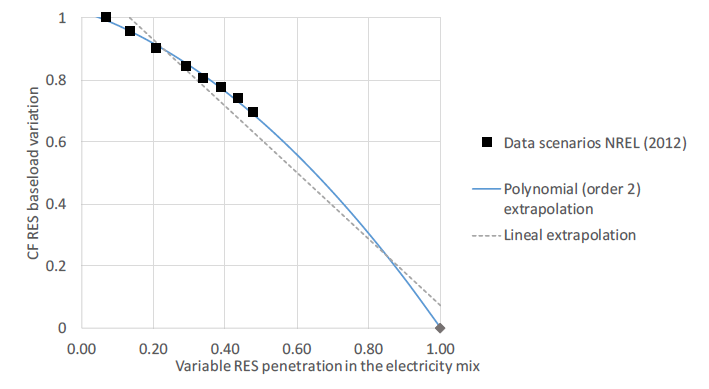
\includegraphics[width=0.8\textwidth]{resources/images/cfres-vreshsare.png}
    \caption{Capacity factor of RES evolution depending on the VRES share \cite{NREL}}
    \label{fig:cfres-vreshare}
\end{figure}

\subsubsection{VRES plants}

MEDEAS based its estimates of the VRES induced overcapacities on \cite{delarue}. These two main impacts of the VRES share are taken into account:
\begin{itemize}
    \item The exponential growth of VRES overcapacities and
    \item The decrease of the VRES capacity factor.
\end{itemize}

The two estimate functions used in MEDEAS \cite{medeas-eroi} from \cite{delarue} are presented on Figure \ref{fig:vres-overcapacities}.

The capacity factor is evaluated as a function of the overcapacity, following Equation \ref{equation:CF}, that can actually be derived from Equations \ref{equation:CF-definition} and \ref{equation:overcapacity}.

\begin{equation}
    CF=\frac{1}{1+overcapacity}
    \label{equation:CF}
\end{equation}

\begin{figure}[h]
    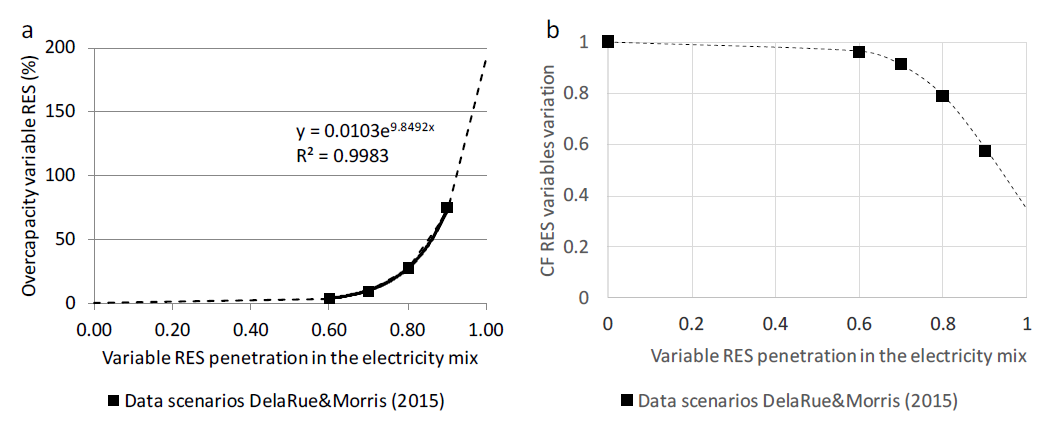
\includegraphics[width=0.9\textwidth]{resources/images/vres-impact-estimate.png}
    \caption{(a) Overcapacity estimate and (b) CF reduction of VRES plants on \cite{medeas-eroi}}
    \label{fig:vres-overcapacities}
\end{figure}

\subsection{Scenarios} \label{section:medeas-scenarios}

As no model can predict with certainty, neither with significant confidence, the decision that will be made and will rule the society for the future, several sets of hypothesis, called scenarios, are made.

When running the MEDEAS model, these scenarios are run in parallel, as in Vensim these are present as possible values for the \textit{scenario} subscript. These possible value have to be chosen in the dedicated panel in Vensim.

By default, the three following scenarios are available, but it is possible to run user-defined scenarios \cite{medeas-website}.

\begin{itemize}
    \item \textbf{BAU} (Business As Usual) corresponds to no particular effort being implemented, the transition continues as it is.
    \item \textbf{OLT} (Optimal Level Transition) where all the resources available are allocated to the best renewable transition possible, that has become a social priority. The only constraints for faster transition are physical limitations.
    \item \textbf{MLT} (Mid-Level Transition) is a mix of the previous ones, some effort are made but not all. Actions towards renewable transition are delayed.
\end{itemize}

A depiction of these scenarios in terms of emissions over time is given on Figure \ref{fig:medeas-scenarios}.

\begin{figure}[h]
    \centering
    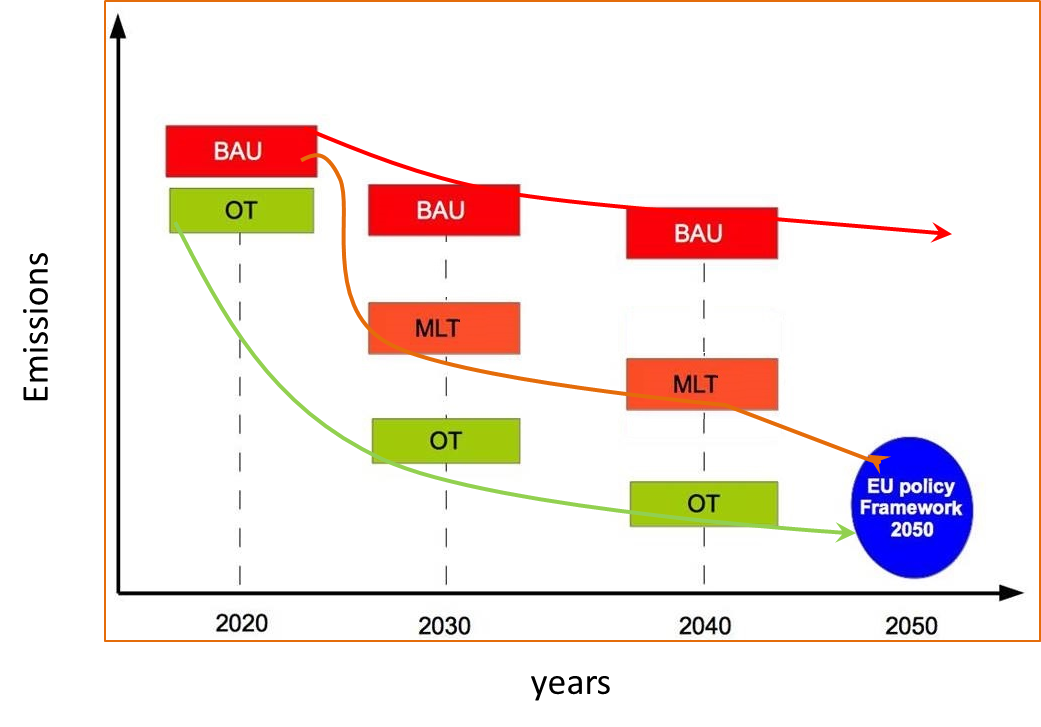
\includegraphics[width=0.8\textwidth]{resources/images/medeas-scenarios.png}
    \caption{Qualitative illustration of the BAU, MLT and OT scenarios for the greenhouse gas emissions in Europe}
    \label{fig:medeas-scenarios}
\end{figure}

These scenarios have been defined somewhat arbitrarily, but the custom scenario capability opens the door to anyone willing to use a more precise, more accurate scenario, given for example additional information brought by major events in the future.